\scanpage{93}
\figure{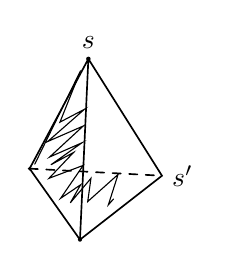
\begin{tikzpicture}[scale=.82,line width=.6pt,line cap=round]
\coordinate (t) at (0,2.1); \coordinate (b) at (-.13,-.7); \coordinate (l) at (-.91,.4); \coordinate (r) at (1.14,.29);
\draw (l)--(t)--(r)--(b)--cycle (t)--(b);
\draw[dashed] (l)--(r);
\draw[thin] (-.83,.47)--(-.12,1.92)--(-.44,1.12)--(-.06,1.32)--(-.63,.82)--(-.08,1.06)--(-.6,.58)--(-.1,.8)--(-.58,.46)--(-.23,.65)--(-.61,.25)--(-.08,.45)--(-.43,-.06)--(-.12,.15)--(-.28,-.13)--(.04,.25)--(-.01,-.11)--(.46,.31)--(.31,-.16)--(.39,-.07);
\fill (t) circle (.035) (b) circle (.032) (l) circle (.03);
\node[above] at (t) {$s$}; \node[right] at (r) {$s'$};
\end{tikzpicture}}
\[
\begin{aligned}
\beta\ \Sigma_r\qquad &(\rho_f,\rho_s,\rho_a) &&\text{\uline{$r$ direct}} &&(3,3,2)^+\\
&(\rho'_f,\rho'_s,\rho'_a) &&\text{\uline{$r$ inverse}} &&(3,3,2)^-\\
&(\rho_s,\rho_{s'},\rho_{s''}) &&(s,s',s'')\ \text{direct \unsure{autour sommet}} &&(3,3,3)^+\\
&(\rho'_s,\rho'_{s'},\rho'_{s''}) &&s,s',s''\ \text{inv. autour \unsure{som}} &&(3,3,3)^-\\
&\underset{\rho_f,\rho_{f'},\rho_{f''}}{\rotatebox{90}{$=$}}
\end{aligned}
\]
\[
\begin{aligned}
\deleted{(\rho_f^{-1},\rho_s,?}\qquad &(3,3,2)^+\longleftrightarrow(3,3,3)^+
  &&(\rho_{\unsure{s+|s|s'}}^{-1},\rho_{\unsure{f+|f|f'}}^{-1},\rho_{\unsure{a|.}}^{-1})\\
\rho_{s'}\qquad &(3,3,2)^-\longleftrightarrow(3,3,3)^-
  &&\underset{\rho_{f'}}{\rotatebox{90}{$=$}}\quad\rho_{s'}\quad
                \underset{\rho_a}{\rotatebox{90}{$=$}}\\
(\rho_f,\underset{\substack{\rotatebox{90}{$=$}\\\rho_{f'}}}{\rho_s^{-1}},?)\qquad
 &(3,3,2)^+\unsure{\mathbin{\text{---}}|\longleftrightarrow|\longleftarrow}(3,3,3)^-\\
 &(3,3,2)^-\longleftarrow(3,3,3)^+
\end{aligned}
\]
\[
\begin{aligned}
\Sigma_r &\qquad \Sigma'_r\\
{\unsure{G|\mathfrak S|\mathcal S}}_3^+\times R &\ \big\backslash\quad \deleted{\unsure{G_3^+}}\times R\\
72&\qquad24\\
\sigma\ \Sigma_r&\ \big|\quad \Sigma'_r\\
\underset{G_3^+}{\rotatebox{90}{$\in$}}\quad\underset{R}{\rotatebox{90}{$\in$}}&
\end{aligned}
\]
\[
\boxed{\sigma\cdot[r]\qquad\unsure{\{r'\}|\{r\}|\{r^{-1}\}}}
\]
\[
\tau\sigma[r]=\sigma^\tau\underline{\tau[r]}
\qquad \tau[r]=\left\{\vphantom{\Large A}\right.
\]
\[
G_3\cdot|\unsure{E|\mathcal E|\mathbb E}|_0\qquad\qquad
\unsure{h|\ell}_0\qquad h_0h_1h_0^{-1}\qquad h_0h_2h_0^{-1}
\]
\diagram{\begin{tikzcd}[ampersand replacement=\&,column sep=small,row sep=small]
\&\Pi_0\arrow[dl,dash]\arrow[r,phantom,"{\underset{\text{inv.}}{\subset}}" description]\&\Omega_0\arrow[d]\arrow[dl,dash]\&\\
{}\arrow[r,dash]\&{\mid}\,|E|_0\&G_3\&\mathbb E\mathrm{l}
\end{tikzcd}}
\[
\begin{aligned}
\rho_1\qquad &\rho_\sigma=\sigma\rho\sigma^{-1}
  &&\underset{-1\quad1}{\rule{1.6em}{.4pt}}\\
&\deleted{\rho_1\rho_\pi\quad\rho'_1\rho'_1}\\
&\overleftrightarrow{\rho_1\rho_2}\quad
  \overleftrightarrow{\rho'_1\rho'_2}\quad\overleftrightarrow{\rho''_1\rho''_2}
  &&\\[-1pt]
&\qquad\underset{\rho_\pi}{\rotatebox{90}{$=$}}
\end{aligned}
\]
\[
\deleted{\rho_1:\ h_0\mathbin{-}h_0^{\unsure{-1}}\quad h_1\longrightarrow}\qquad\rho_1
\]
\[
\begin{aligned}
&\tikz[baseline=(a.base)]{\node (a) {$\rho_1\rho''_2$}; \draw (a.center) ellipse (2.1em and .8em);}\\
&\tikz[baseline=(b.base)]{\node (b) {$\rho'_1\rho_2$}; \draw (b.center) ellipse (2.1em and .8em);}\\
&\tikz[baseline=(c.base)]{\node (c) {$\rho''_1\rho'_2$}; \draw (c.center) ellipse (2.1em and .8em);}
\end{aligned}
\]
\[
\begin{aligned}
x+y+z\ &=0\\
-x+y+&
\end{aligned}
\qquad
\begin{array}{cccccc}
(-1,\unsure{1|0},\unsure{-1|1})&(1,-1,-1)&(-1,-1,\unsure{1|0})&
(\unsure{1|0},-1,-1)&(0\ 0,-1)&(-1,0\ 0)\\[-1pt]
\multicolumn{6}{c}{\rule{.4pt}{.45em}\rule{.75\linewidth}{.4pt}\rule{.4pt}{.45em}}\\[-2pt]
\rho_1&\rho_2&\rho'_1&\rho'_2&\rho''_1&\rho''_2
\end{array}
\]
% archive sheet number: 92
